%--------------------------------------------CAPA DE NEGOCIOS ------------------------------------------------------%

\subsection{Capa de negocios}
Los elementos de la capa empresarial se utilizan para modelar la \textbf{organización operativa} de una empresa de manera independiente de la tecnología, mientras que los elementos estratégicos se utilizan para modelar la dirección estratégica y las opciones de la empresa.

La tabla \ref{tab:Tabla de la capa de negocios} ofrece una descripción general de los elementos de la capa empresarial, con sus definiciones.\cite{archimate} 

\begin{longtable}{|p{0.15\linewidth}|p{0.45\linewidth}|p{0.2\linewidth} p{0.2\linewidth}|}
    \caption{Tabla de la capa de negocios}
    \\
    \hline
    \rowcolor[HTML]{AFC5F6} 
    \textbf{Elemento} & \textbf{Descripción} & \multicolumn{2}{c|}{\textbf{Notación}} \\
    \hline
    \endhead
    \hline
    \multicolumn{4}{r}{\textit{Continúa en la siguiente página}} \\
    \endfoot
    \hline
    \endlastfoot
    \label{tab:Tabla de la capa de negocios}
    %Contenido 1 &
    %\lipsum[1] &
    %Datos A1
    %& Datos B1
    %\\
    %\hline



    Actor comercial 
    &
    Representa una entidad comercial  que es capaz de realizar un comportamiento.
    &
\begin{center}
    
\includegraphics[width=1\linewidth]{imgs/capa_de_negocios/1.pdf}
\end{center} 
&
\begin{center}
    
\includegraphics[width=0.3\linewidth]{imgs/capa_de_negocios/a1.pdf}
\end{center}
    \\ \hline



    Rol comercial 
    &
    Representa la responsabilidad de realizar un comportamiento específico, al que se puede asignar un actor, o el papel que juega un actor en una acción o evento particular.
    &
\begin{center}
    
\includegraphics[width=1\linewidth]{imgs/capa_de_negocios/2.pdf}
\end{center} &
\begin{center}
    
\includegraphics[width=0.5\linewidth]{imgs/capa_de_negocios/a2.pdf}
\end{center}
    \\ \hline



    Colaboración comercial
    &
    Representa un agregado de dos o más elementos de la estructura interna activa de la empresa que trabajan juntos para realizar un  comportamiento colectivo.
    &
\begin{center}
    
\includegraphics[width=1\linewidth]{imgs/capa_de_negocios/3.pdf}
\end{center} &
\begin{center}
    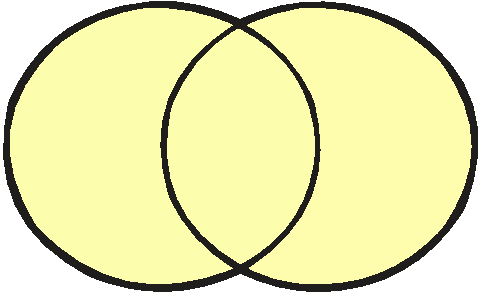
\includegraphics[width=0.5\linewidth]{imgs/capa_de_negocios/a3.pdf}
\end{center}
    \\ \hline



    Interfaz comercial
    &
    Representa un punto de acceso donde los servicios comerciales se ponen a disposición del entorno.
    &
\begin{center}
    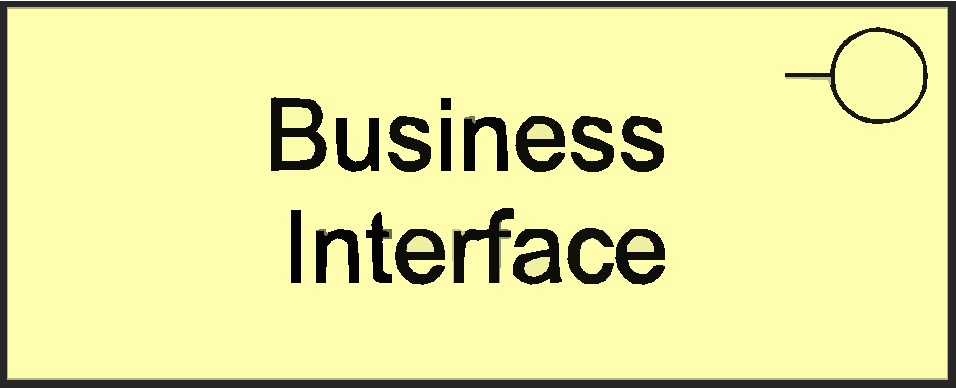
\includegraphics[width=1\linewidth]{imgs/capa_de_negocios/4.pdf}
\end{center} &
\begin{center}
    
\includegraphics[width=0.5\linewidth]{imgs/capa_de_negocios/a4.pdf}
\end{center}
    \\ \hline

    Proceso comercial
    &
    Representa una secuencia de comportamientos comerciales que logra un resultado específico, como un conjunto definido de productos o servicios comerciales.
    &
\begin{center}
    
\includegraphics[width=1\linewidth]{imgs/capa_de_negocios/5.pdf}
\end{center} &
\begin{center}
    
\includegraphics[width=0.5\linewidth]{imgs/capa_de_negocios/a5.pdf}
\end{center}
    \\ \hline


    Función comercial
    &
    Representa una colección de comportamiento comercial basado en un conjunto elegido de criterios, como los recursos comerciales necesarios y/o las competencias, y se gestiona o realiza como un todo.
    &
\begin{center}
    
\includegraphics[width=1\linewidth]{imgs/capa_de_negocios/6.pdf}
\end{center} &
\begin{center}
    
\includegraphics[width=0.5\linewidth]{imgs/capa_de_negocios/a6.pdf}
\end{center}
    \\ \hline

    Interacción comercial
    &
    Representa una unidad de comportamiento comercial colectivo realizado por (una  colaboración de) dos o más actores comerciales, roles comerciales o colaboraciones comerciales.
    &
\begin{center}
    
\includegraphics[width=1\linewidth]{imgs/capa_de_negocios/7.pdf}
\end{center} &
\begin{center}
    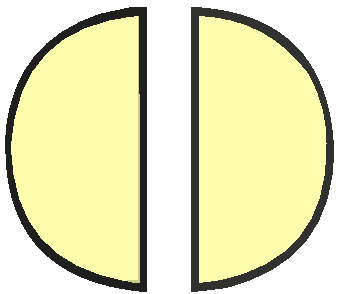
\includegraphics[width=0.5\linewidth]{imgs/capa_de_negocios/a7.pdf}
\end{center}
    \\ \hline


    Evento comercial
    &
    Representa un cambio de estado relacionado con el negocio.
    &
\begin{center}
    
\includegraphics[width=1\linewidth]{imgs/capa_de_negocios/8.pdf}
\end{center} &
\begin{center}
    
\includegraphics[width=0.5\linewidth]{imgs/capa_de_negocios/a8.pdf}
\end{center}
    \\ \hline

    Servicio comercial
    &
    Representa explícitamente el comportamiento definido que un rol comercial, un actor comercial o una colaboración comercial expone a su entorno.
    &
\begin{center}
    
\includegraphics[width=1\linewidth]{imgs/capa_de_negocios/9.pdf}
\end{center} &
\begin{center}
    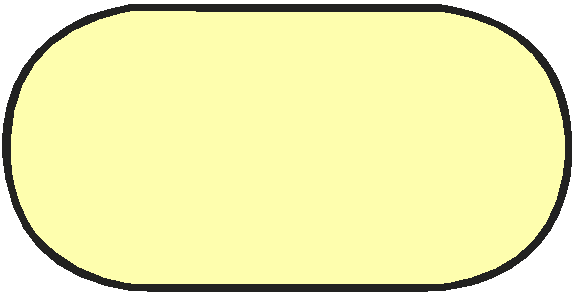
\includegraphics[width=0.5\linewidth]{imgs/capa_de_negocios/a9.pdf}
\end{center}
    \\ \hline

    Objeto comercial
    &
    Representa un concepto utilizado dentro de u dominio comercial particular.
    &
\begin{center}
    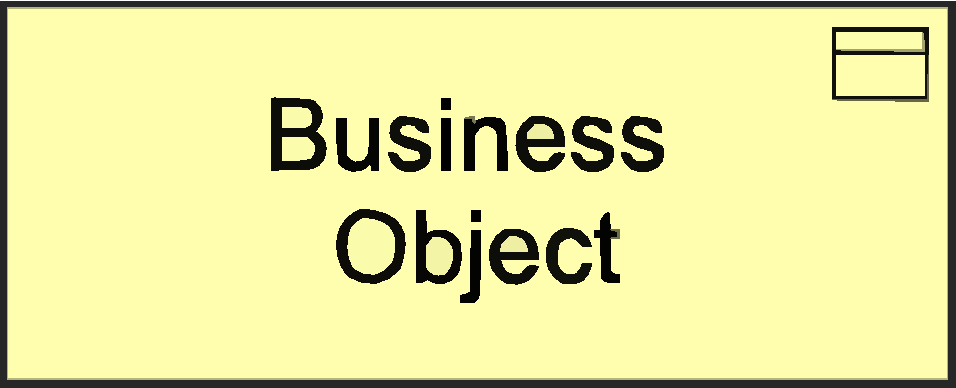
\includegraphics[width=1\linewidth]{imgs/capa_de_negocios/10.pdf}
\end{center} &
\begin{center}
    
\includegraphics[width=0.5\linewidth]{imgs/capa_de_negocios/a10.pdf}
\end{center}
    \\ \hline

    Contrato
    &
    Representa una especificación formal o informal de un acuerdo entre un proveedor y u consumidor que especifica los derechos y obligaciones asociados con un producto y establece parámetros funcionales y no funcionales para la interacción.
    &
\begin{center}
    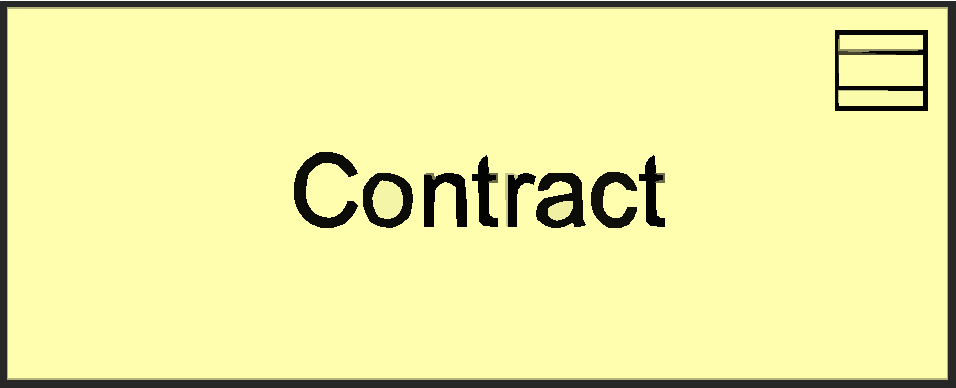
\includegraphics[width=1\linewidth]{imgs/capa_de_negocios/11.pdf}
\end{center} &
\begin{center}
    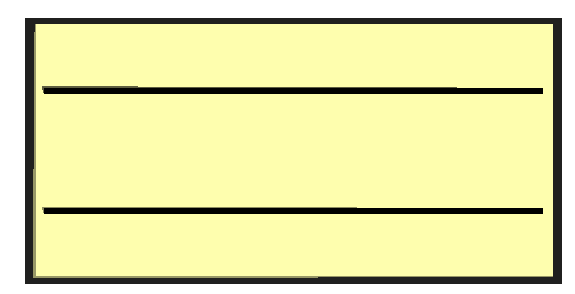
\includegraphics[width=0.5\linewidth]{imgs/capa_de_negocios/a11.pdf}
\end{center}
    \\ \hline

    Representación
    &
    Representa una secuencia de comportamientos comerciales que logra un resultado específico, como un conjunto definido de productos o servicios comerciales.
    &
\begin{center}
    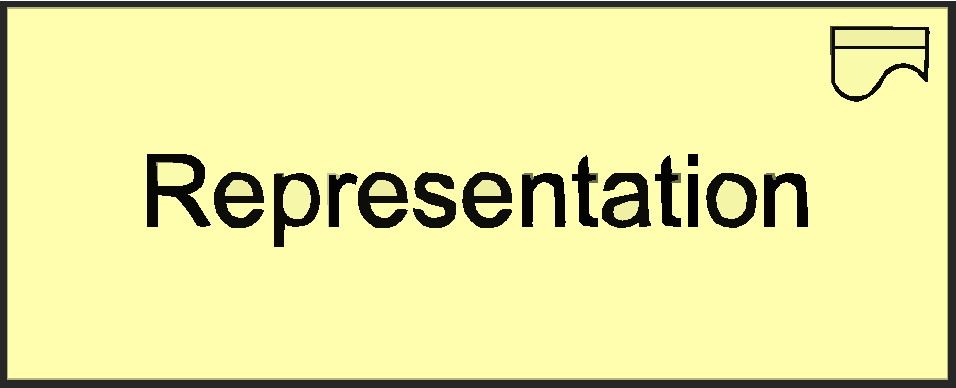
\includegraphics[width=1\linewidth]{imgs/capa_de_negocios/12.pdf}
\end{center} &
\begin{center}
    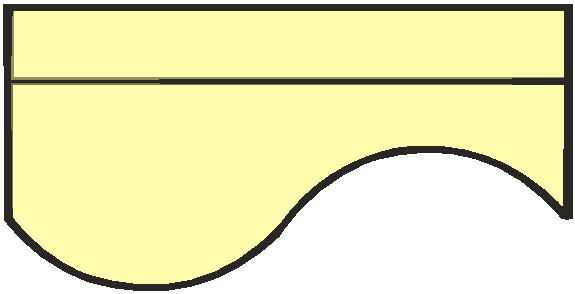
\includegraphics[width=0.5\linewidth]{imgs/capa_de_negocios/a12.pdf}
\end{center}
    \\ \hline

    Producto
    &
    Representa una forma perceptible de la información que lleva un objeto de negocio.
    &
\begin{center}
    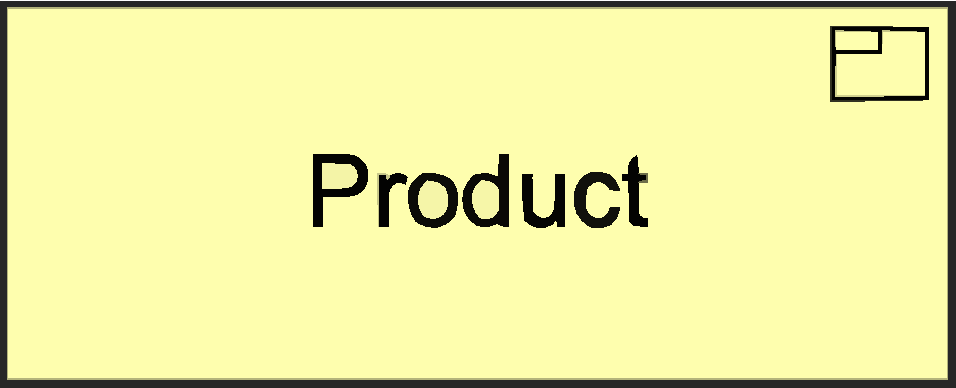
\includegraphics[width=1\linewidth]{imgs/capa_de_negocios/13.pdf}
\end{center} &
\begin{center}
    
\includegraphics[width=0.5\linewidth]{imgs/capa_de_negocios/a13.pdf}
\end{center}
    \\ \hline


\end{longtable}